\chapter{相关理论与技术}\label{chap:theories_tech}

\section{Linux调度子系统}

% 内核Core调度流程
% 影响内核调度的关键因素
% - HZ
% - 调度类/机制
% - 调度策略/算法
% - 高质量的操作系统组件,如调度器,则可能需要数十年的时间来完善\citep{agache2020firecracker}

调度子系统是Linux内核的一个重要组成部分,主要负责在多任务场景中为每个任务分配CPU资源。Linux调度子系统在架构上可分为如图~\ref{fig:sched_arch}所示三层,各层为上层提供了基本机制,各层协作为复杂调度机制的实现提供了可能。其中,最底层的Sched Core层提供了基本的调度框架,包括抢占调度与非抢占调度。Sched Class层则针对不同调度目标,提供了包括实时调度、公平调度等特性,并且不同的调度类间存在优先级差异。最上层的Sched policy则考虑到不同任务的优先性,在调度类的基础之上进一步实现优先级调度。具体而言,Fair调度类基于Sched Core实现了公平调度,并提供NORMAL与BATCH两种的调度策略,用于区别地调度优先性更低的批处理任务。

\begin{figure}[!htbp]
    \centering
    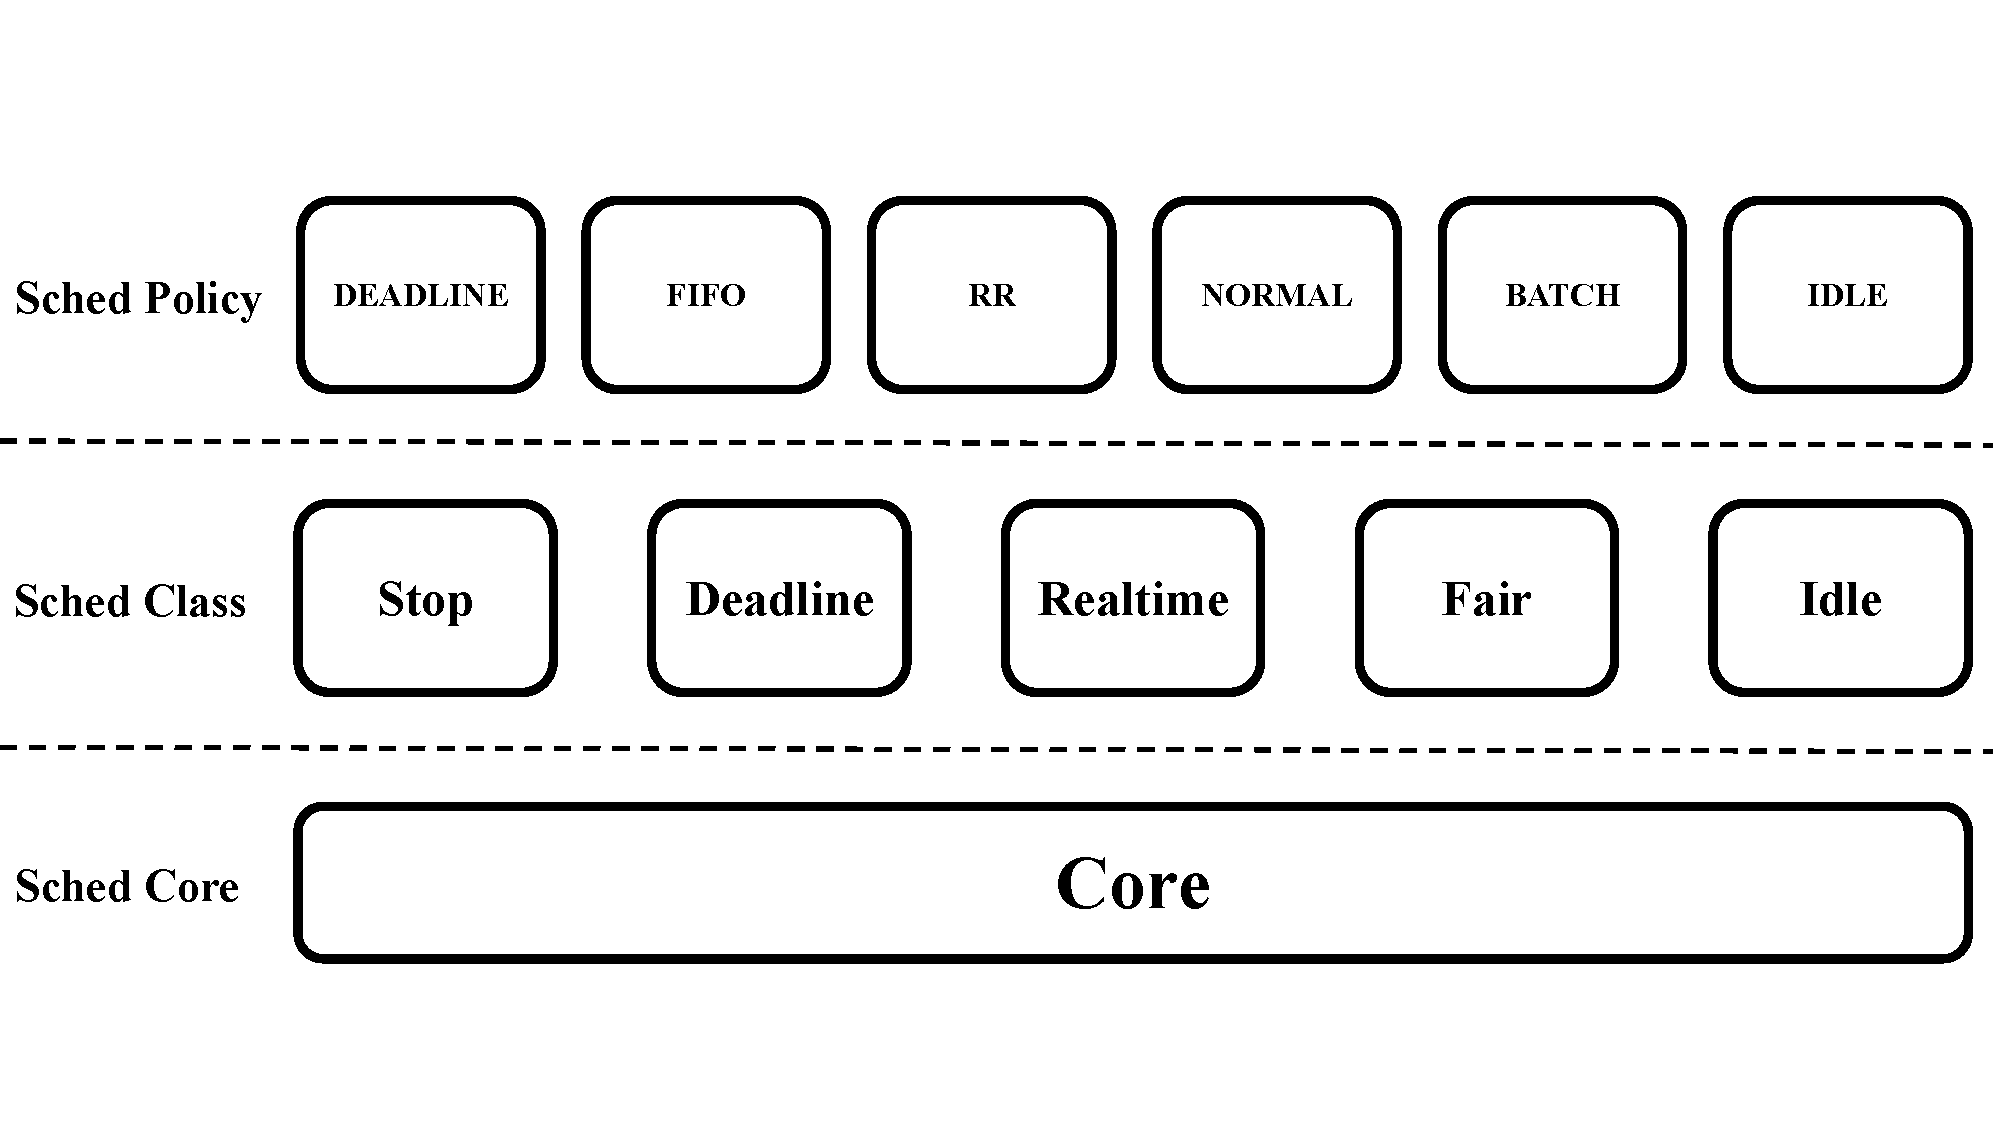
\includegraphics[width=0.8\textwidth]{sched_arch}
    \bicaption{\quad 调度子系统架构}{\quad Scheduling subsystem architecture}
    \label{fig:sched_arch}
\end{figure}

Sched Core层作为最基本的调度框架,是所有调度机制的基本入口。Core调度可分为非抢占式调度与非抢占式两个部分,其中非抢占式调度起源于批处理调度,在这一场景中,任务依次执行直到退出,如图~\ref{fig:schedule_core}所示,Core调度器需要为新fork出来的任务选择合适的CPU并进行入队,而当任务exit或主动出让CPU之后,则需要进行出入队管理,选择下一个继续的任务,并执行任务切换。而从上一个任务切换到下一个任务的过程即是调度循环,如图~\ref{fig:shcedule_loop}所示,调度循环通常由中断和系统调用驱动,并在处理完毕到返回用户任务之前的时刻,判断标志位来决定是否进入到调度循环。抢占式调度基于CPU的分时复用,一般由时钟中断驱动,如图~\ref{fig:schedule_tick}所示,在时钟中断处理函数中,会触发Core中的task\_tick,在其中就包含了当前任务所属调度类的响应回调,如更新当前任务的记账信息,以及决策是否进行抢占等。实际的抢占通过Core提供的resched\_curr实现,对于任务所在的CPU而言,该函数设置了抢占标记位,从而在时钟中断处理完毕后触发调度循环来完成任务的抢占。

\begin{figure}[!htbp]
    \centering
    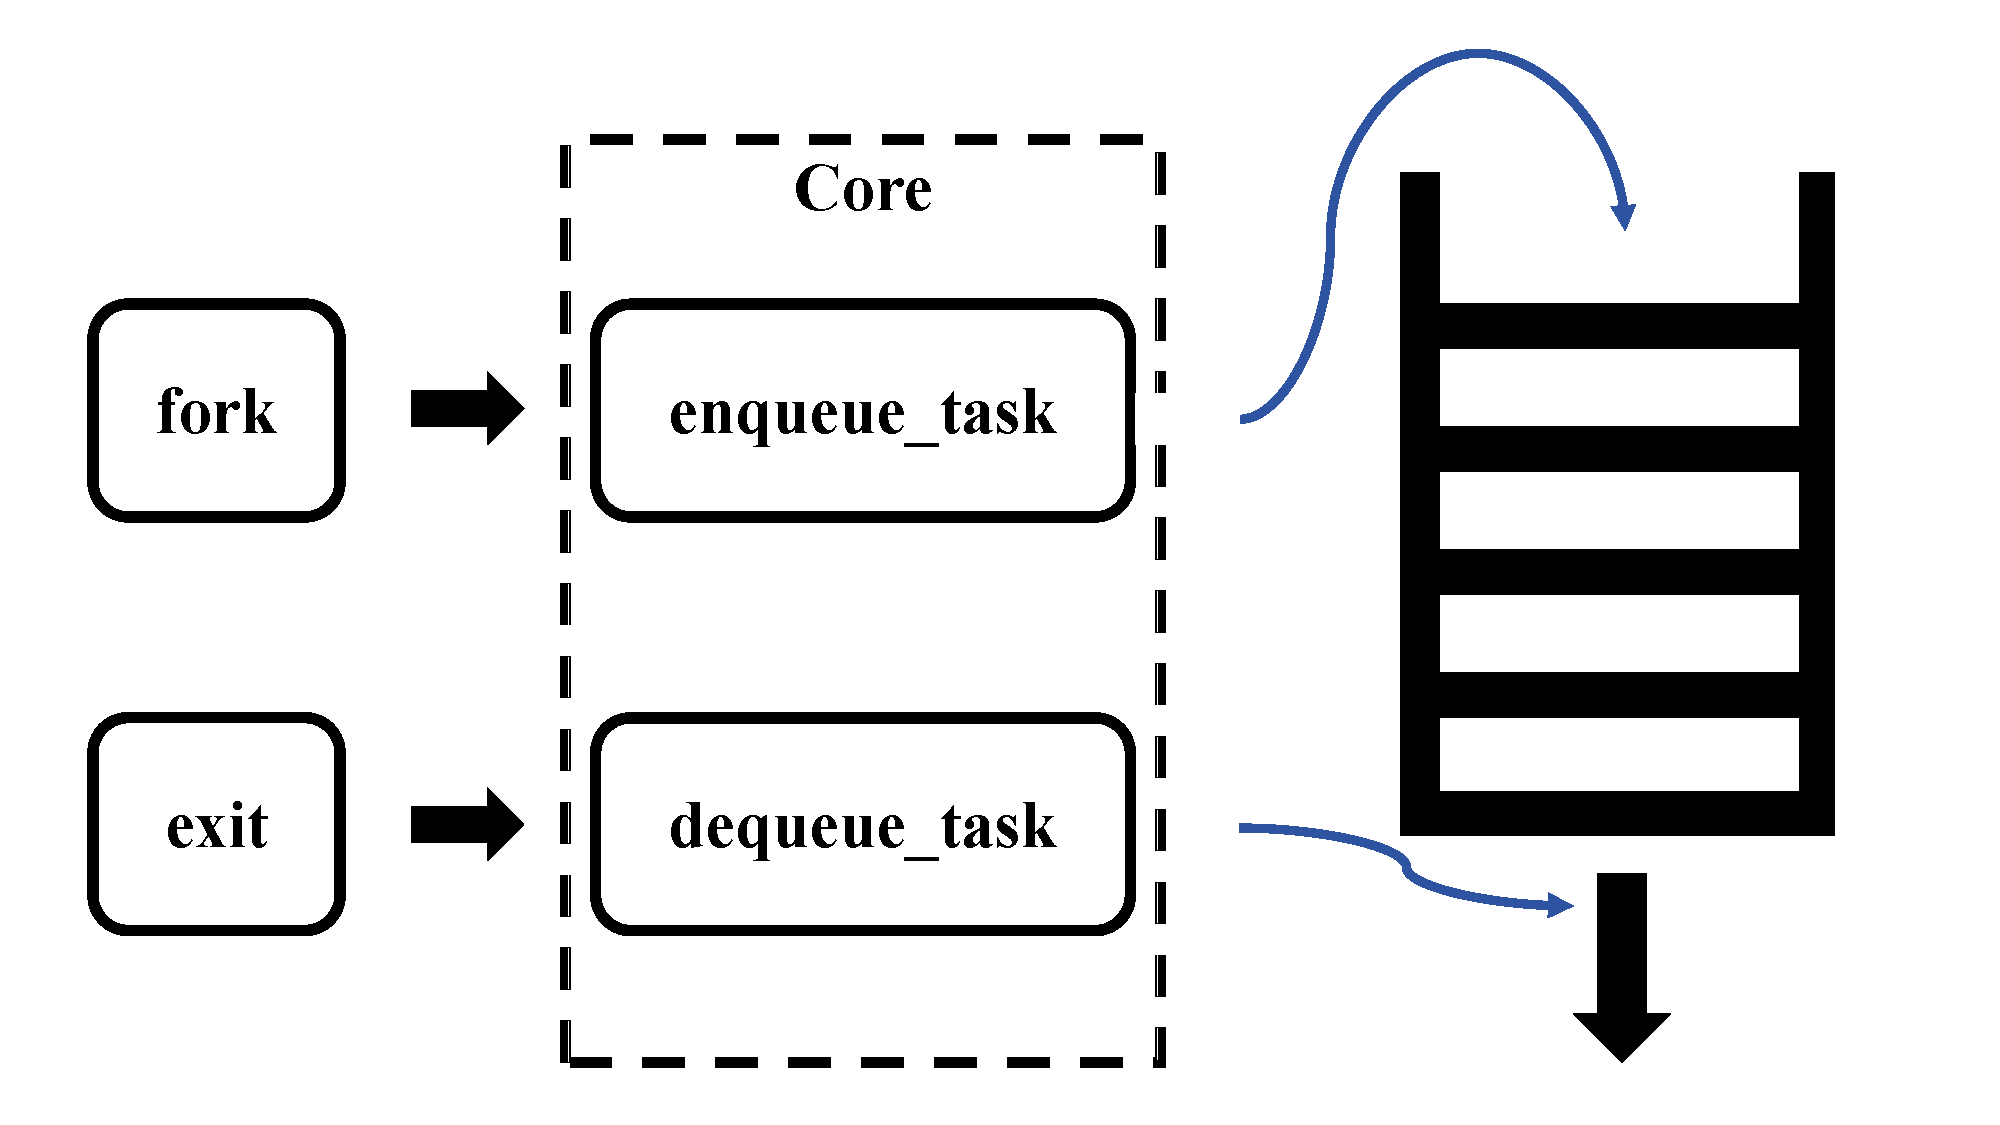
\includegraphics[width=0.5\textwidth]{schedule_core}
    \bicaption{\quad Core任务调度}{\quad Core scheduling tasks}
    \label{fig:schedule_core}
\end{figure}

Sched Class调度类层基于Core调度框架实现。当前Linux中主要包含Stop、Deadline、Realtime、Fair、Idle五大调度类\citep{scheduler}。其中,Stop调度类的实现最简单,其本质上是从批处理调度中提出出来的逻辑。Fair调度类最复杂,使用到如红黑树等高级数据结构,并采用了较复杂的启发式算法与记账逻辑,力图以公平作为调度的目标,而其在多数场景下的稳定性能使得Fair长久以来都作为Linux中任务的默认调度类。其余调度类同样以不同的目标进行设计,如Deadline调度类能够保证任务在设定的周期中执行固定的时间。Linux为这些调度类设置的固定的优先级, 每个调度循环都会从最高优先级的调度类开始尝试获取任务,这使得属于较高优先级调度类的任务总是能被优先执行。

\begin{figure}[!htbp]
    \centering 
    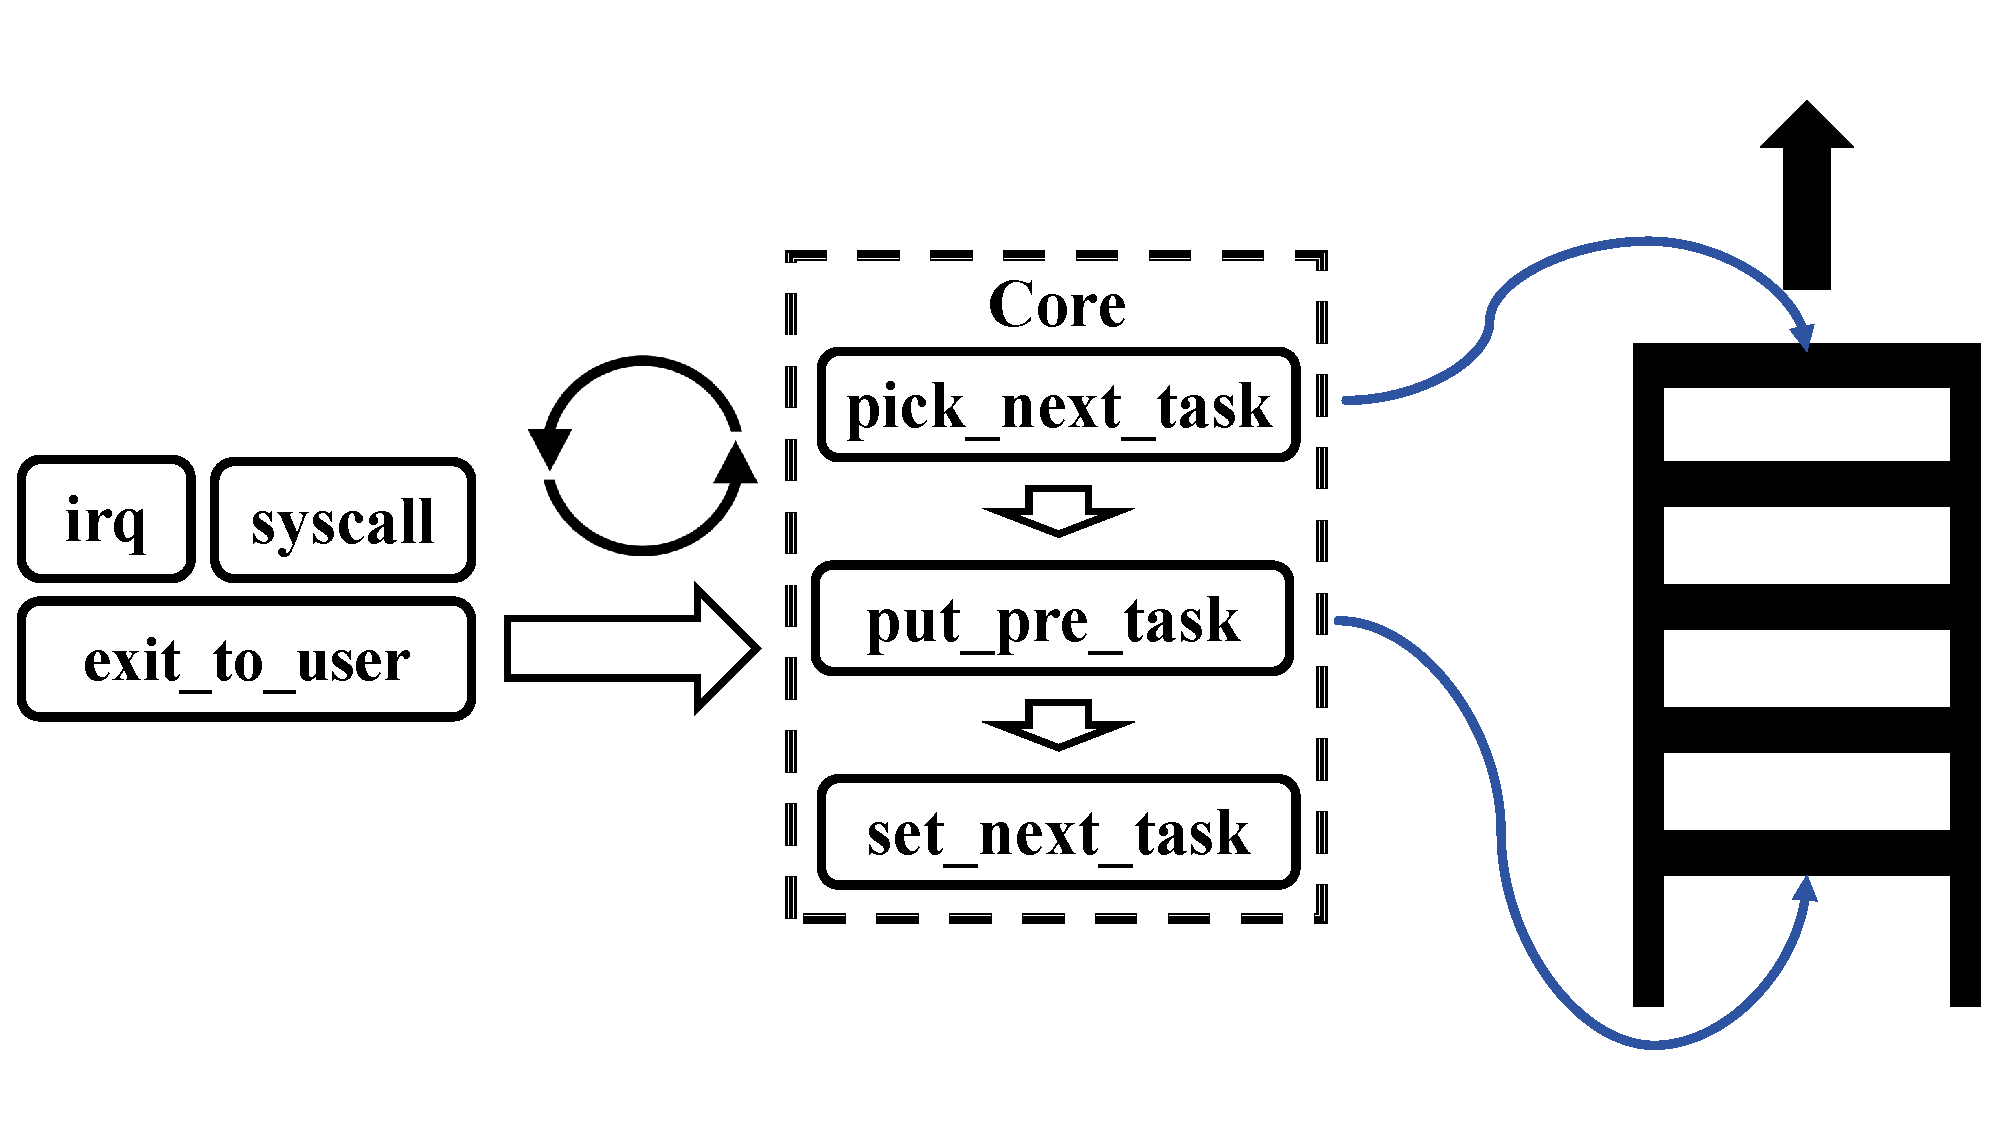
\includegraphics[width=0.6\textwidth]{shcedule_loop}
    \bicaption{\quad 调度循环}{\quad Schedule Loop}
    \label{fig:shcedule_loop}
\end{figure}

Sched Policy调度策略层基于调度类层实现,主要处理调度队列中的优先级机制,不同调度类中的实现各不相同。在Realtime调度类中,优先级体现为多个调度队列,选取任务时会从最高优先级的任务队列开始,这保证了高优先级的任务被优先执行,而在同一个任务队列中,调度策略则区分了任务轮换的形式,如FIFO采用先来先执行的逻辑,而RR则通过时间片轮转依次执行任务。在Fair调度类中,优先级机制的实现则完全不同,这种差异性来自于Fair调度类的算法实现上,如CFS调度算法会为每个任务维护一个vruntime,并优先选择vruntime最小的任务执行,在CFS算法中,优先级体现为vruntime积累的差异,高优先级的任务积累vruntime的速度会更慢,从而获取更多的执行机会,基于如上设计,Fair调度类提供了NORMAL与BATCH两种调度策略,对应为不同的优先级,来适配不同类型任务的调度场景。

\begin{figure}[!htbp]
    \centering
    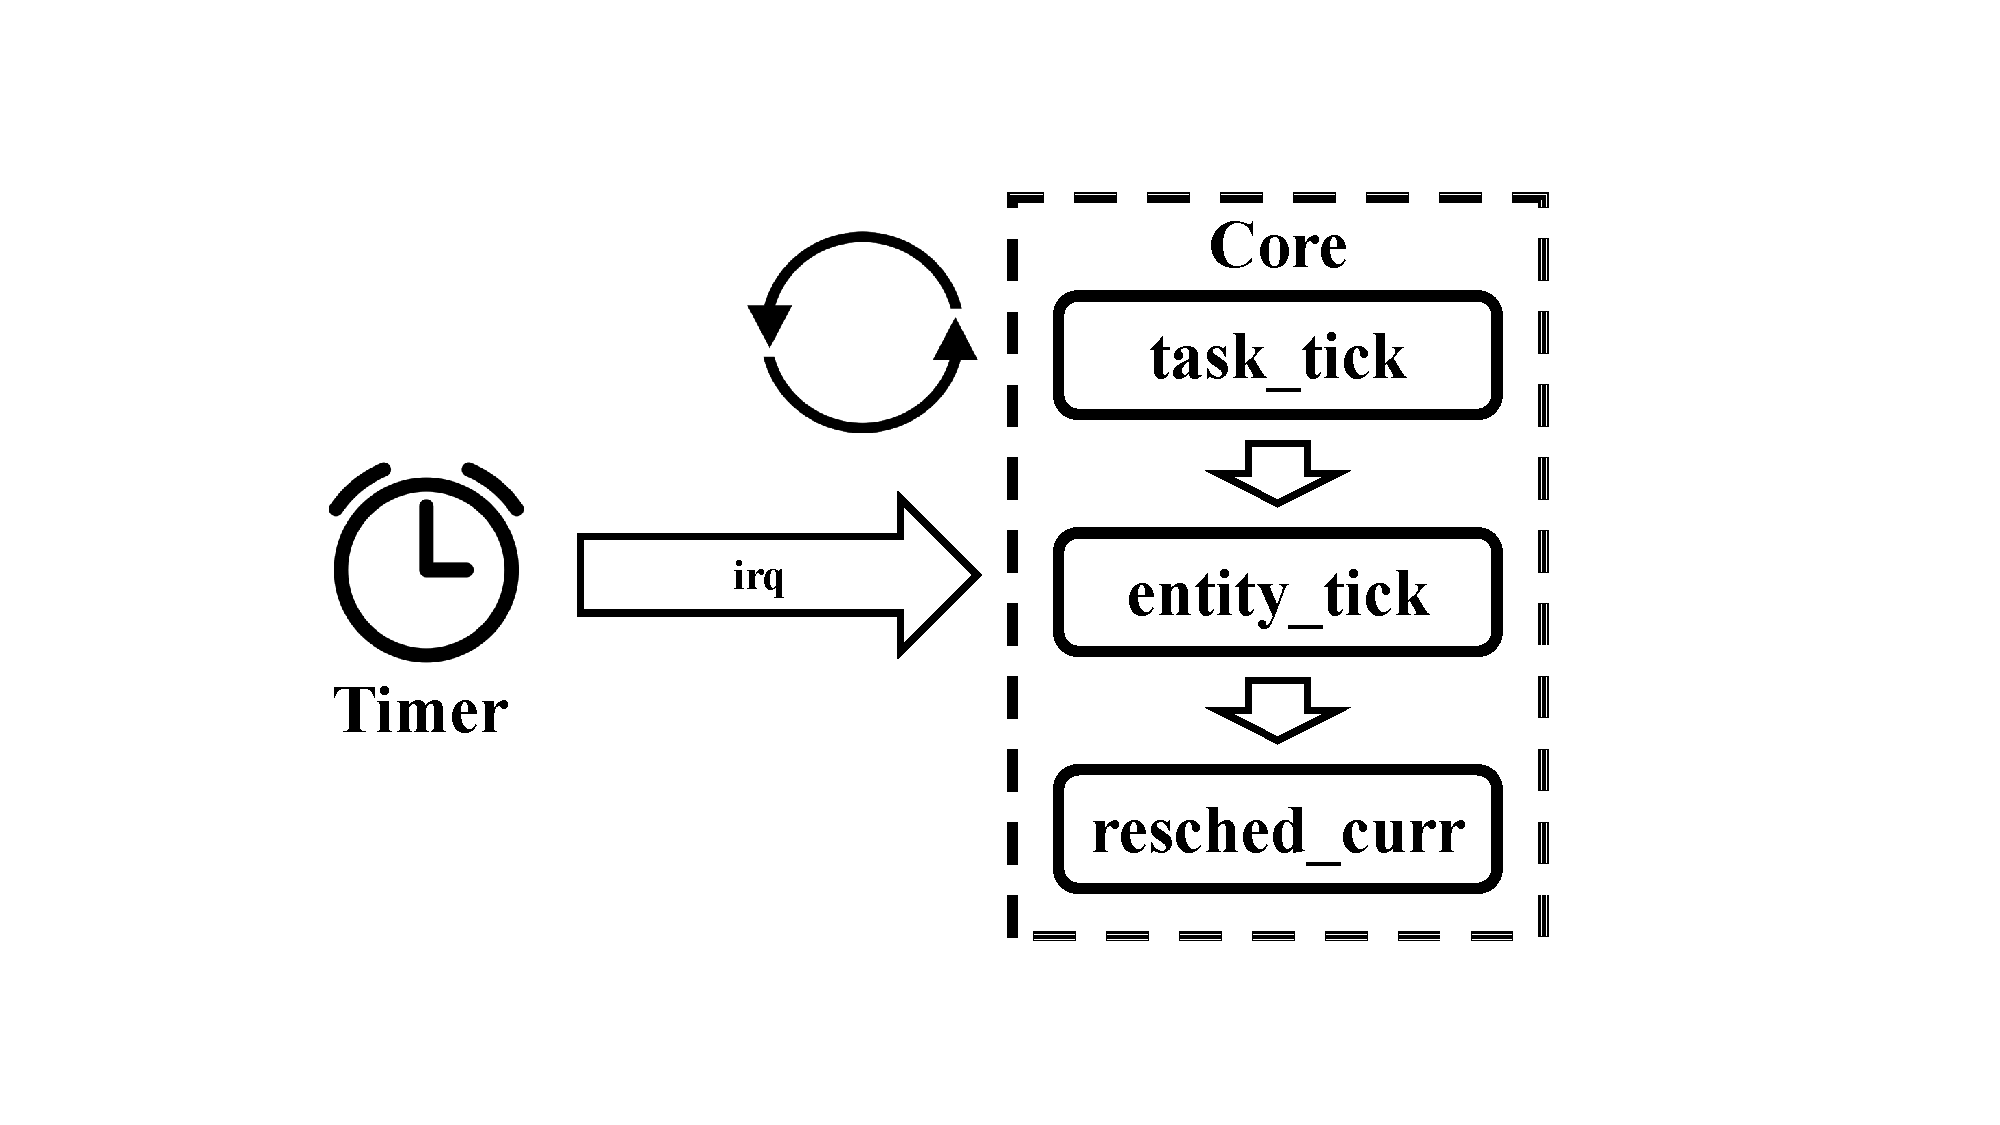
\includegraphics[width=0.5\textwidth]{schedule_tick}
    \bicaption{\quad 抢占调度时钟滴答}{\quad Schedule Tick}
    \label{fig:schedule_tick}
\end{figure}

\section{BPF技术}

% 定制内核的需求: 多样的硬件/多样的网络处理模式
% 内核模块: 灵活性高,但不安全,容易引发内核crash风险
% BPF在网络子系统引入,自定义网络包的处理流程
% 逐渐拓展到各个子系统中,但由于内核的审慎地设计,其他子系统中通常用来进行只读操作,如进行监测

eBPF(Extended Berkeley Packet Filter)是一个运行在Linux内核中的轻量、高效64位的类RISC虚拟机\citep{sharaf2022extended}。eBPF凭借其强大的性能,以及在可移植性、灵活性与安全性的优势,得到了工业界和学术界的广泛认可,并逐渐成为在Linux内核中执行不可信的、由用户定义的专用代码的最佳实践与事实标准。

eBPF的前身是BPF(Berkeley Packet Filter),最早由McCannel和Jacobson提出\citep{mccanne1993bsd},用于在Linux网络子系统中实现用户自定义的网络包处理。BPF优异的设计与理念得到了Linux社区贡献者的广泛认可,并逐渐扩展到除网络子系统以外的其他子系统中。而为进行区分,Linux社区将早期的BPF技术称为cBPF(Classic Berkeley Packet Filter)。当前BPF与eBPF均指代最新的BPF技术,本文后续说明中也沿用此做法。

BPF虚拟机包含10个通用寄存器以及1个只读的帧指针寄存器,位宽均为64-bits。与JVM类似,BPF虚拟机采用字节码作为执行指令的格式,并定义了一套完整的指令集。BPF字节码作为一种中间语言,解耦了编译环境与执行环境,在实现可移植性的同时保证了性能。另一方面,BPF字节码相较于机器码来说语义更明确,便于Linux内核进行验证,从而减少未定义行为的代码进入内核,提升安全性。

早期BPF程序仅支持使用BPF汇编编写,当前随GCC、Clang等主流编译器对BPF字节码的支持,开发者可以使用C、Rust等高级语言开发BPF程序\citep{ebpfguidence}。出于安全性的考量,BPF并非是图灵完备的,开发者通常只能使用高级语言的子集来进行BPF程序的开发。编译好的BPF程序是一个常规的ELF文件,支持二次修改来进一步提升灵活性。BPF程序最终运行在Linux内核的BPF虚拟机中,相关过程依赖一系列系统调用完成。负责BPF程序加载的系统调用中,首先,Linux内核会尝试运行BPF程序来检验其中是否存在非法的部分,如越界的内存访问、不确定的循环等。随后,对于合法的BPF程序,Linux内核会将其保存到一段指定的内核内存空间中,并附加到指定的内核插桩点处。此后每次到达插桩点时,就会跳转至BPF虚拟机并对附加的BPF程序进行解释执行。

BPF技术通常会与同样作为内核功能扩展的内核模块比较,而相较于内核模块,BPF技术的优势体现在更高的安全性上,主要体现在两个方面:

\begin{enumerate}
    \item BPF程序的编写有严格的限制。一方面,BPF并非图灵完备的,因此程序逻辑通常较为简单,并一定程度上减少未定义行为的出现。另一方面,Linux内核会在BPF程序加载时进行验证,并拒绝加载非法的BPF程序,从而避免执行不安全的代码。
    \item BPF程序与内核的交互是受控的。内核模块与内核的交互通过直接的函数与变量访问实现,而不做限制的交互模式存在较大的安全风险。相反,BPF程序仅允许通过BPF Helper函数来与内核交互,包括对内核数据的读写、共享内存使用等。BPF Helper函数限制了BPF程序所能访问的内核功能,以达到受控的交互。其次,部分BPF Helper函数保证线程安全,提供基本的安全性保证。最后,BPF程序所能附着的插桩位点由内核提供,因此BPF程序的影响范围也是受内核控制的。
\end{enumerate}

% TODO: 修改图例
\begin{figure}[!htbp]
    \centering
    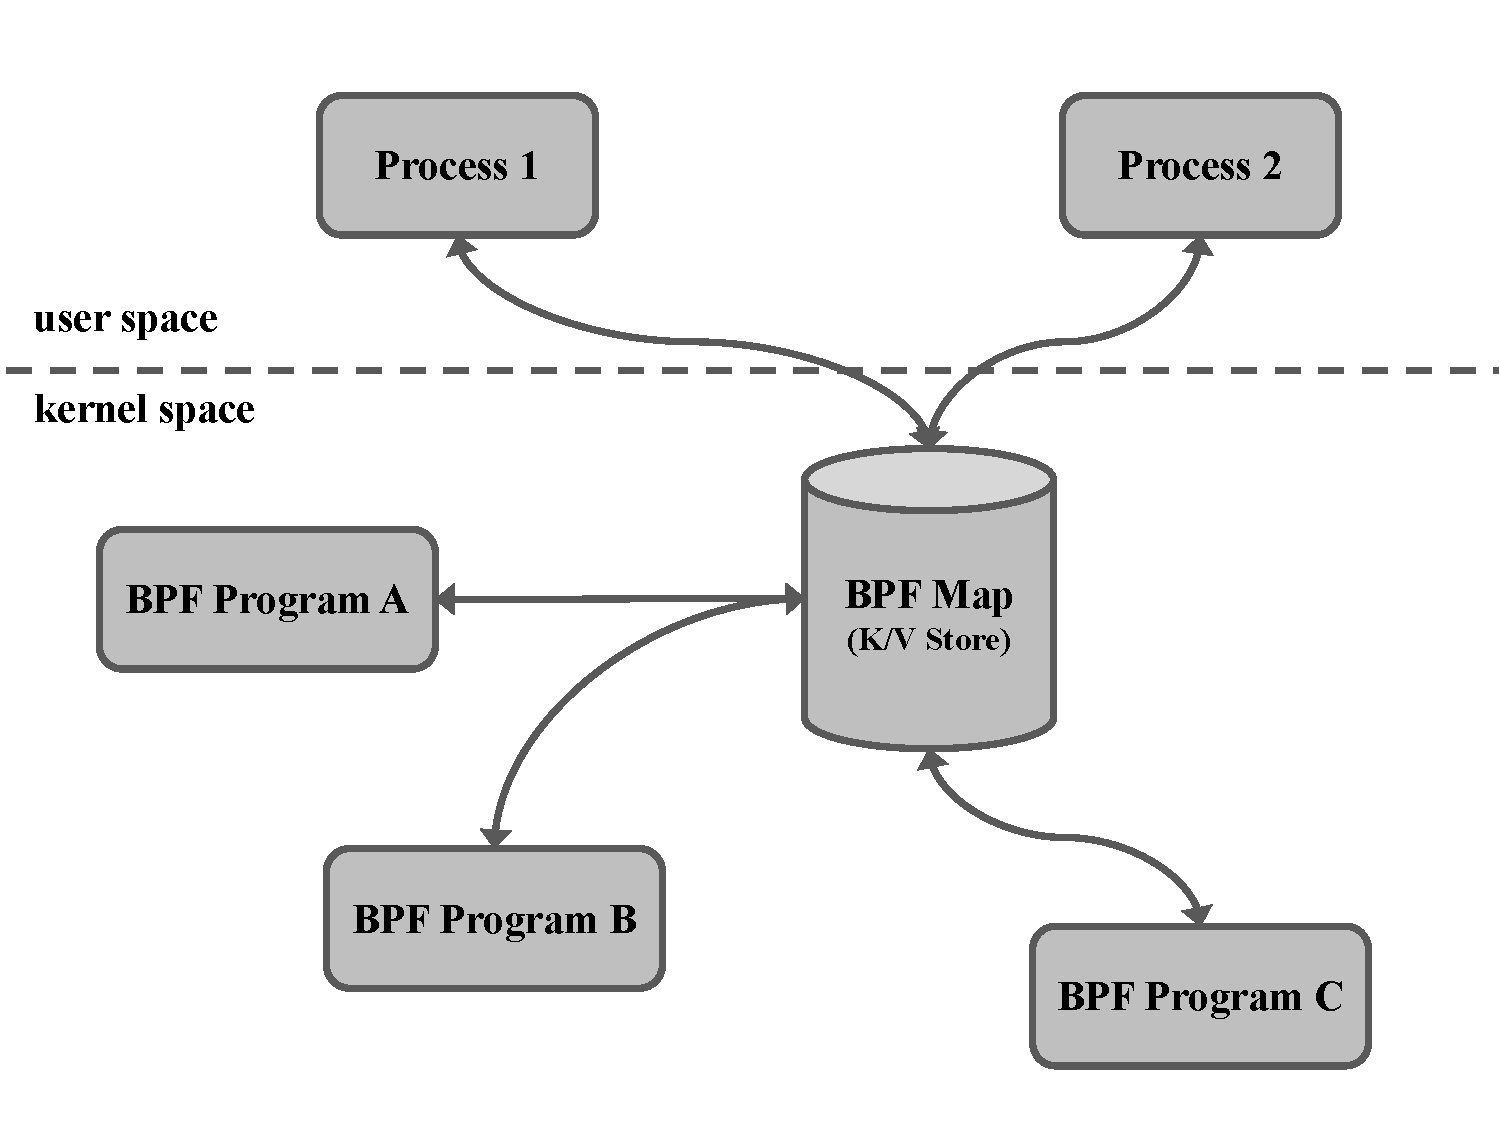
\includegraphics[width=0.6\textwidth]{bpf_user_kernel}
    \bicaption{\quad BPF中用户态与内核态的交互}{\quad Interaction between user mode and kernel mode in BPF}
    \label{fig:bpf_user_kernel}
\end{figure}

BPF技术具有高度的灵活性。首先,开发者可以利于libbpf等库来对BPF程序进行操作,如读写BPF程序中的全局变量、选择性地加载部分BPF程序等。其次,BPF程序中可以通过如图~\ref{fig:bpf_user_kernel}所示的BPF Map实现共享内存。一方面,用户程序可以通过BPF Map来安全地读写内核数据,如读取BPF程序采集的信息或者修改BPF程序的行为。另一方面,BPF程序之间可以通过BPF Map实现彼此之间的协作。最后,BPF程序之间也能够进行如图~\ref{fig:bpf_to_bpf}所示的相互调用,突破内核对单个BPF函数的限制,实现更复杂的逻辑。

% TODO: 修改图例
\begin{figure}[!htbp]
    \centering
    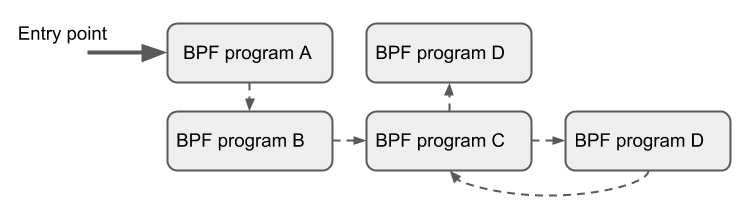
\includegraphics[width=0.7\textwidth]{bpf_to_bpf}
    \bicaption{\quad BPF程序之间的调用}{\quad Interaction between BPF programs}
    \label{fig:bpf_to_bpf}
\end{figure}

BPF程序通常在加载后由BPF虚拟机进行解释执行,这种相对低效的执行方式会对内核性能产生一定的影响。为提升BPF程序的执行效率,Linux内核提供了BPF JIT配置选项,允许在BPF代码加载时将字节码直接编译为本机的机器码。同时,在插桩点触发时,也不再是由BPF虚拟机解释执行,而是在捕获到内核的栈上数据之后,直接的跳转到编译为机器码的BPF程序处执行。BPF JIT使得BPF程序的执行效率大大提高。

BPF技术在设计上也存在一些不足。首先,编写BPF程序所能使用的C语言的子集并非是图灵完备的,因此无法实现较为复杂的逻辑,同时BPF程序在栈空间上也有严格的要求,这些都与BPF子系统在安全与开销上设计目标一致,但是较弱的语言表达性往往使得BPF的使用场景有限。其次,BPF运行在内核环境中,依赖BPF Helper函数而不是系统调用来与内核沟通,而现行内核中Helper通常设计为针对有限的子系统受限制地开放,这也进一步限制了BPF程序的功能。不过,BPF技术在灵活性与安全性上的优势仍得到了内核开发者以及云原生社区的重视。如Linux内核社区中的BPF-next SIG就致力于解决BPF技术当前的种种问题,并尝试逐步减少对BPF程序的限制,以及在各个子系统中扩展BPF程序的功能。

BPF技术开源社区维护十分积极,当前主流生态可分为BCC(BPF Compiler Collection)\citep{bcc}与libbpf\citep{libbpf}两支:

\begin{enumerate}
    \item BCC提供了基于Pyhton语言的BPF元编程框架。框架中,开发者只需要定义少量的BPF程序文本,而完整的BPF代码生成、内核兼容性、编译环境选择均由BCC完成。实际BCC包含了完整的BPF编译环境,并在运行时自动识别目标机器的内核来进行BPF程序编译河加载。BCC元编程框架大大减少了BPF程序的开发难度,同时选择在目标机器上进行编译,也有利于解决迁移时的内核兼容性问题。然而这种方式一方面引入了额外的编译环境开销,另一方面编程框架的过度封装也不利于BPF新特性的快速接入。
    \item libbpf采用CO-RE(Compile Once – Run Everywhere)的思想。CO-RE即在本地就将BPF编译为字节码并保存为只读数据。开发者可以通过libbpf提供一系列辅助函数读写编译好的BPF程序,并利用库函数完成BPF程序的加载、附加及卸载。相较于BCC,使用libbpf开发的BPF项目在空间占用上更小,同时也不需要在目标机器上进行编译,因此能够做到在不同机器上快速部署。而为解决内核版本的兼容性问题,一方面开发者可以借助bpftool工具来获取目标内核中的数据结构信息,从而编译得到适用目标内核版的BPF程序。另一方面,开发者可以在BPF程序中声明兼容性,从而指导内核加载的过程。
\end{enumerate}

\section{可扩展调度类}

Sched Ext可扩展调度类项目\citep{schedext},最早于2022年由Meta工程师提出,用来解决Meta数据中心对调度的需求与Linux内核调度修改难、迭代慢的矛盾。Sched Ext项目的整体架构如图~\ref{fig:sched_ext_arch}所示,主要包含两个部分,其中内核部分为Ext调度类补丁集,由Meta工程师与内核社区工作者共同维护,当前尚未合入内核主线,用户态部分包含BPF Scheduler开发框架,基于Libbpf封装并支持C与Rust语言。Sched Ext项目当前已经在Meta集群中部署与测试,同时项目社区更新十分活跃。

\begin{figure}[!htbp]
    \centering
    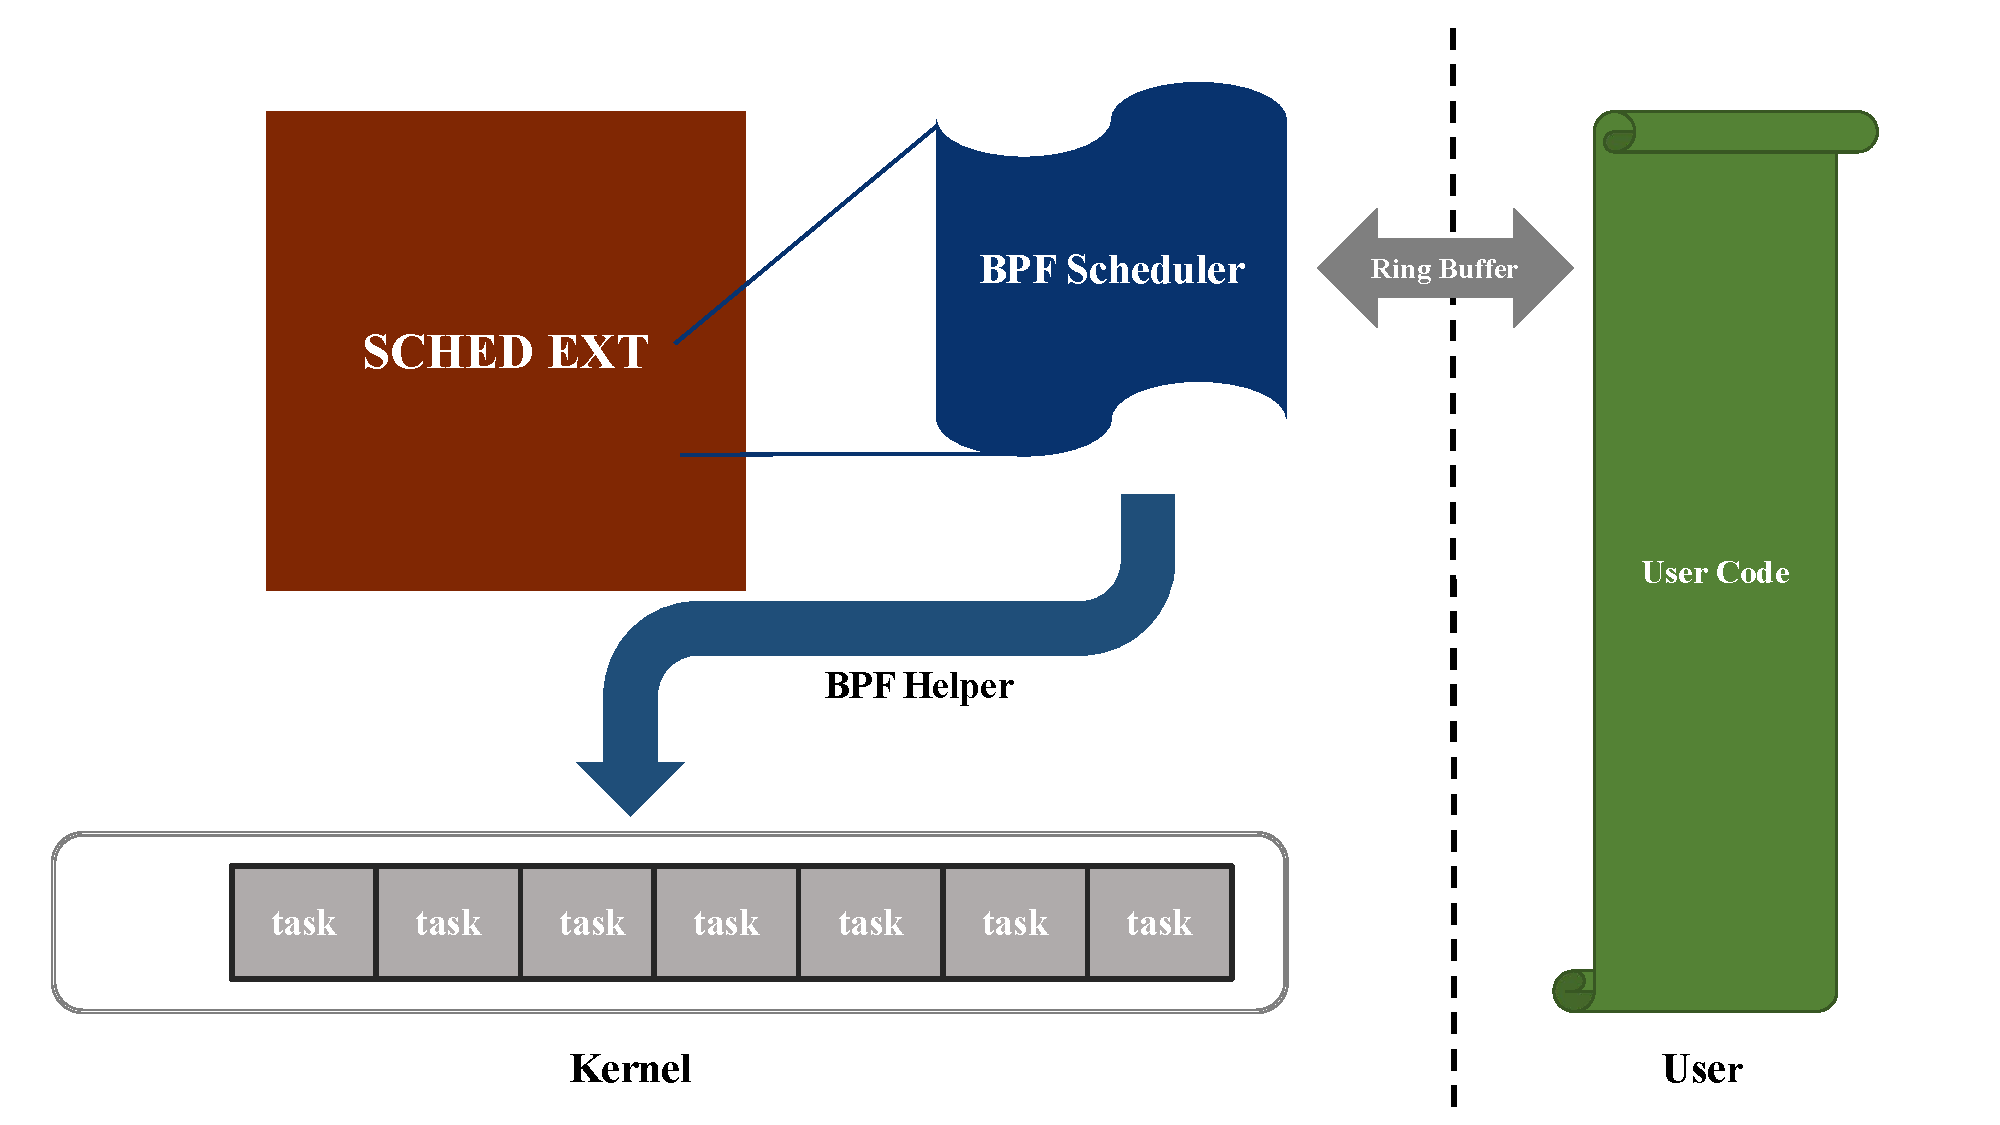
\includegraphics[width=0.75\textwidth]{sched_ext_arch}
    \bicaption{\quad Sched Ext架构}{\quad Sched Ext Arch}
    \label{fig:sched_ext_arch}
\end{figure}

Sched Ext项目启发自ghOSt\citep{humphries2021ghost},通过设计一种插件化的调度类来提升Linux内核调度子系统开发的灵活性。在实现灵活的调度类上,Sched Ext与ghOSt存在两点主要差异,首先,Ext调度类在设计之初就尽可能地保持与Linux现有调度子系统的兼容性,如图~\ref{fig:sched_ext_priorty}所示,Ext调度类在优先级上有意地放置在Fair调度类与Idle调度类之间,当Ext调度类没有管理任务时,Linux调度子系统能够保持原有的所有特性,而当前Ext调度类管理了任务时,调度类会判断当前是否存在BPF Scheduler,并在BPF Scheduler没有加载时将任务交给Fair调度类处理,综合以上设计,Ext调度类做到对现有调度子系统的最小干扰。其次,Sched Ext项目使用BPF技术作为调度类扩展性的实现机制,相较于系统调用,一方面,BPF Scheduler能够保持在内核态运行,实现更小的调度开销,另一面,BPF本身就具有足够的表达能力,能够实现大部分的调度逻辑,同时BPF支持丰富的用户态交互手段,从而支持更灵活的用户态调度逻辑的表达。

\begin{figure}[!htbp]
    \centering
    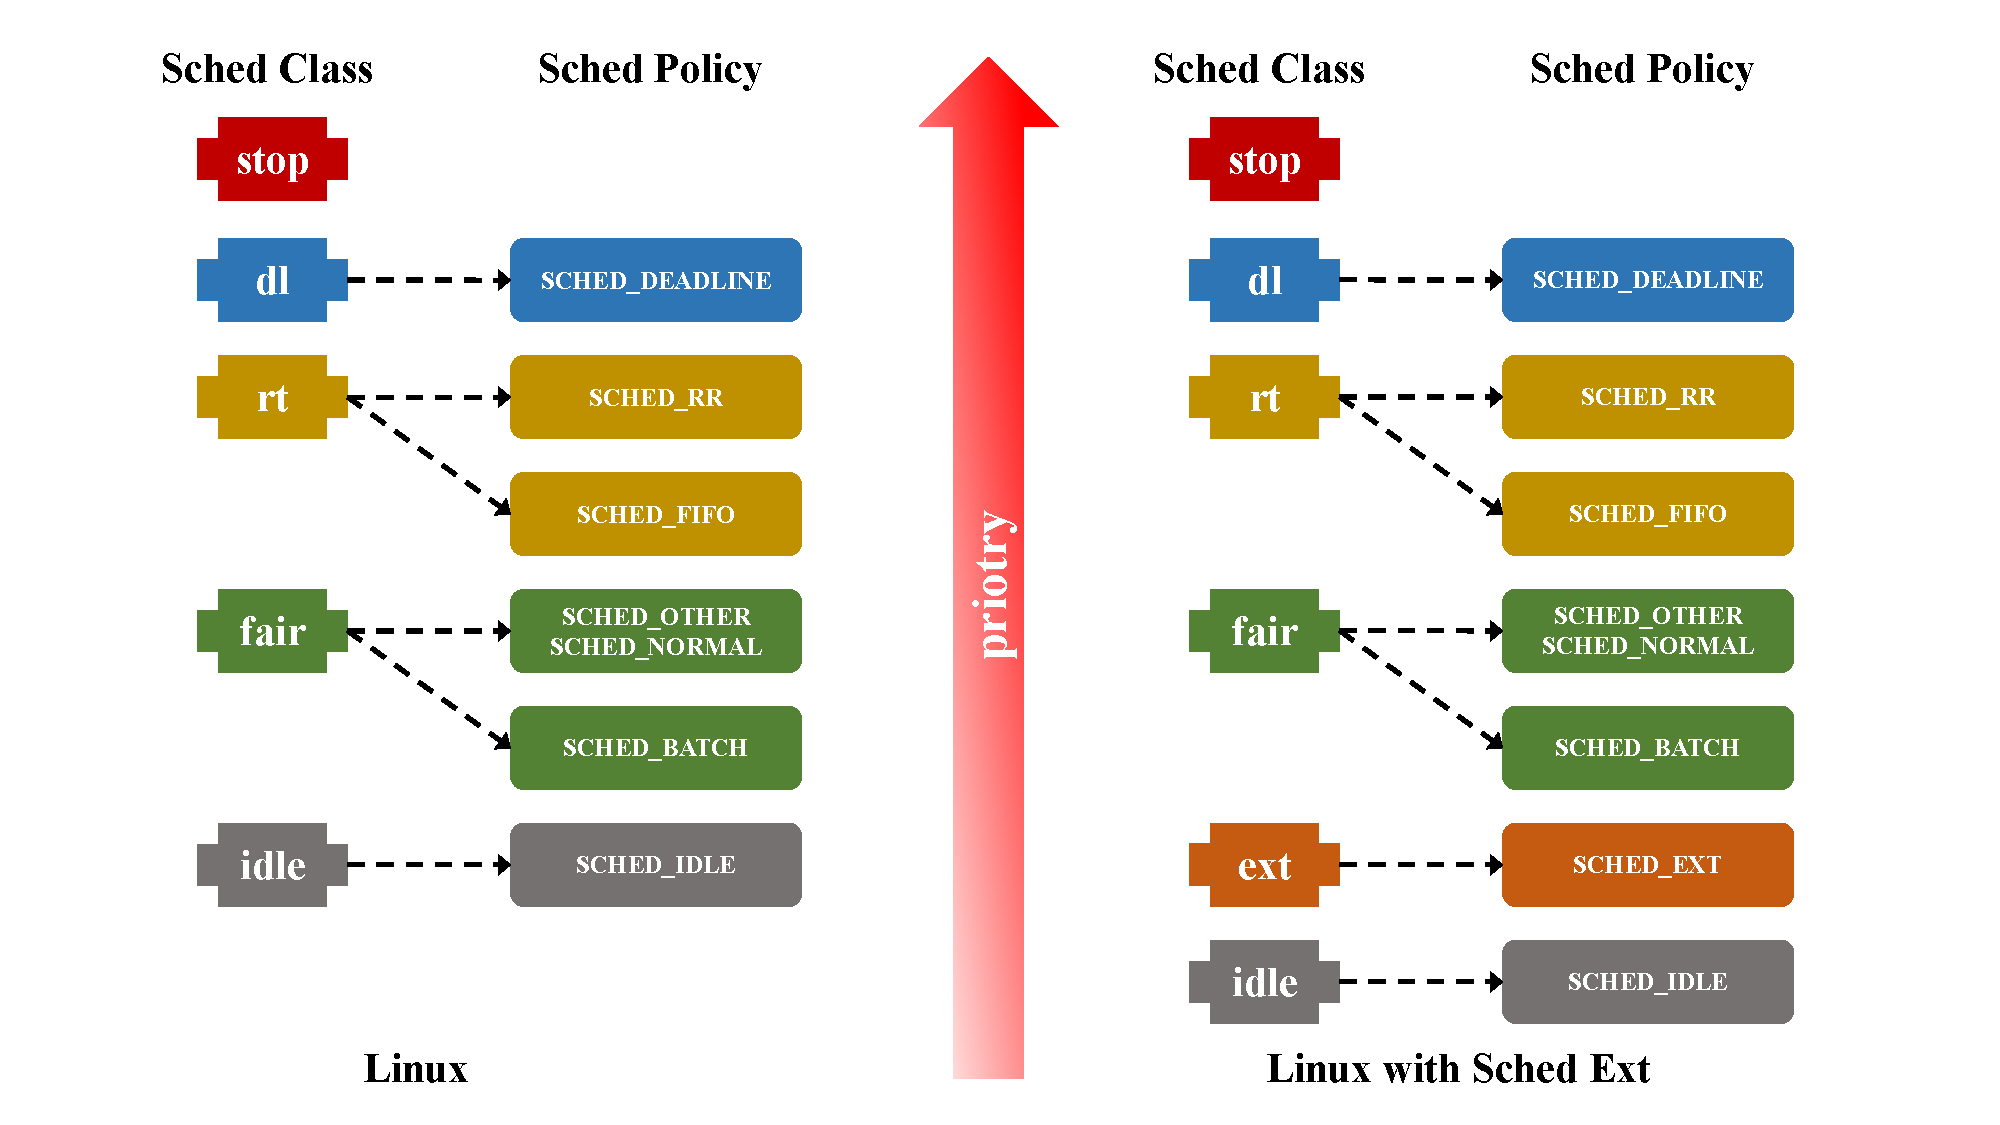
\includegraphics[width=0.9\textwidth]{sched_ext_priorty}
    \bicaption{\quad Sched Ext 调度优先级}{\quad Sched Ext Priorty}
    \label{fig:sched_ext_priorty}
\end{figure}

Ext调度类实现了sched\_class的完整方法并注册在内核调度子系统中。相较于其他调度类,Ext调度类的最大特点是调度的过程需要与BPF Scheduler协作完成。如图~\ref{fig:sched_ext_helpers}所示,为实现Ext调度类与BPF Schedule的交互,在数据通路上,Sched Ext项目提供了DSQ(Dispatch Queue),用于保存和传递任务,Ext调度类在初始化时,会为每个CPU创建一个Local DSQ,Ext调度类所管理的CPU需要从Local DSQ中获取任务并执行,BPF Scheduler也可以有自己的DSQ,用于在BPF程序中对任务进行管理,BPF Scheduler调度的底层逻辑就是BPF DSQ与Local DSQ之间任务的流转。在控制通路上,Sched Ext项目增加了一系列BPF Helper函数,主要包括DSQ的管理以及BPF Scheduler与CPU之间的交互,具体功能如下:

\begin{itemize}
    \item \textbf{scx\_bpf\_create\_dsq}: 定义一个DSQ(调度队列)来对任务进行管理。DSQ是BPF Scheduler管理任务的核心, BPF程序中可以保有不止一个DSQ,DSQ之间通过ID来进行区分,同时通过NUMA亲和性能够来保证访问DSQ内存的效率。
    \item \textbf{scx\_bpf\_dispatch、scx\_bpf\_dispatch\_vtime}:将任务调度到DSQ中。调度逻辑中可通过ID来指定目标DSQ以及任务的运行slice,其中slice可以设置为无限,此时任务不会被同队列中的其他任务抢占,而由BPF程序来决策抢占的时机。调度的任务通常以FIFO的形式入队,Sched Ext也提供了基于vtime的类CFS队列,以满足不同的BPF调度器的设计需求。

    \begin{figure}[!htbp]
        \centering
        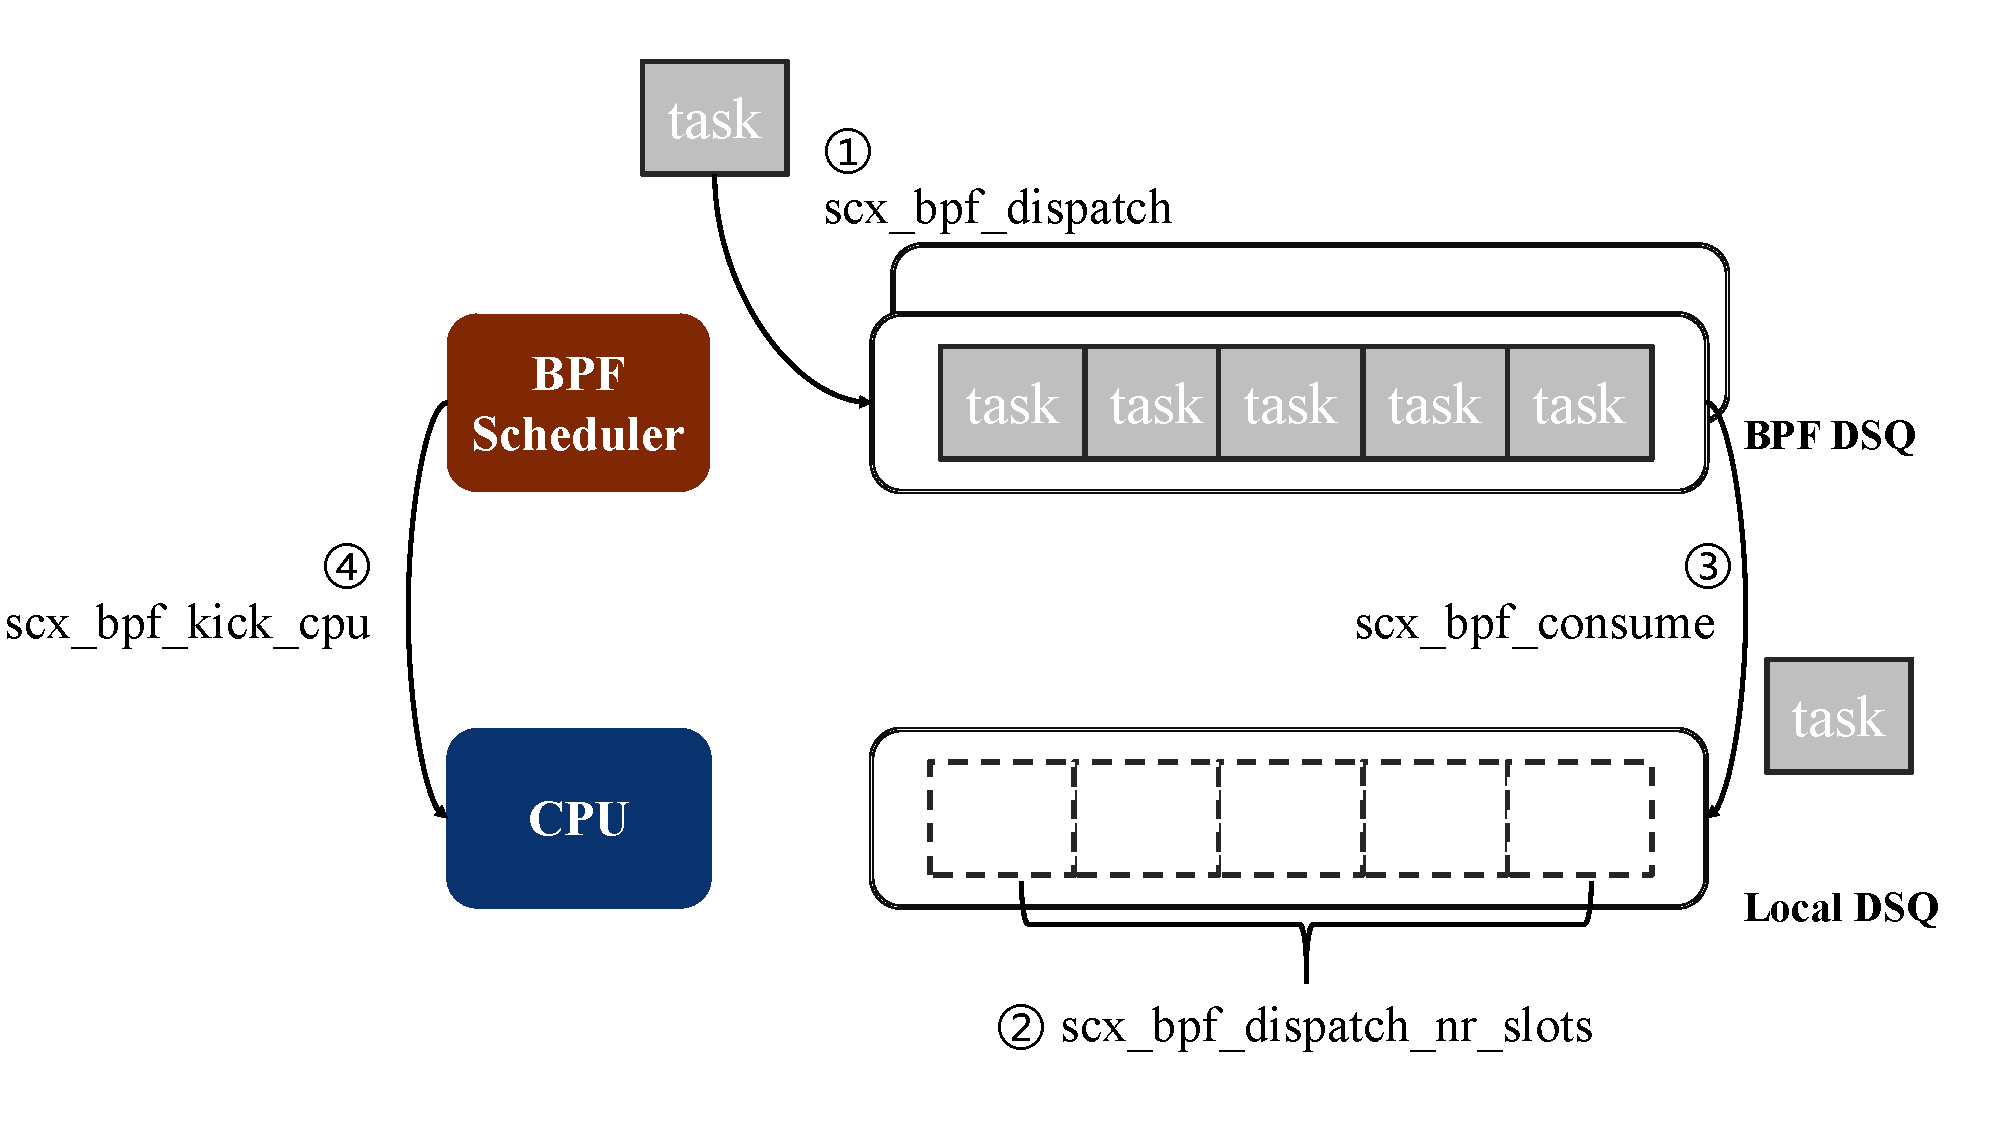
\includegraphics[width=0.85\textwidth]{sched_ext_helpers}
        \bicaption{\quad Sched Ext BPF Helper 函数}{\quad Sched Ext BPF Helpers}
        \label{fig:sched_ext_helpers}
    \end{figure}
    
    \item \textbf{scx\_bpf\_dispatch\_nr\_slots}:查看CPU可调度的任务槽数。允许BPF程序检查当前CPU上可承载的任务余量,避免BPF Scheduler向目标CPU调度过多的任务。
    \item \textbf{scx\_bpf\_dispatch\_cancel}:撤销最近向CPU调度的一个任务。当任务的CPU亲和性发生变化时,BPF Scheduler原先调度的任务就应当进行变化,而此Helper函数便于BPF Scheduler撤销先前的调度决策。
    \item \textbf{scx\_bpf\_consume}:将BPF scheduler管理的任务调度给CPU。Sched Ext中的任务需要经过从BPF Scheduler的调度队列到CPU本地调度对队列的过程,这一过程的通过此Helper函数完成。
    \item \textbf{scx\_bpf\_kick\_cpu}:激活CPU的重调度。BPF程序能够通过此Helper函数唤醒一个idle CPU或者让繁忙的CPU进入调度循环中,为避免唤醒过程对调度延迟的影响,因此采用向中断队列添加延时任务的形式异步地设置唤醒任务,而在唤醒的过程主要通过Core框架提供的resched\_curr函数完成。
    \item \textbf{scx\_bpf\_pick\_idle\_cpu}:找到一个空闲的CPU。根据不同的调度目标,调度器应当避免任务过度的集中于同一个CPU,BPF Scheduler可以通过此Helper函数找到一个空闲CPU,将任务调度到此CPU上,并结合其他Helper函数来唤醒CPU。
\end{itemize}

Ext调度类与BPF Scheduler的关系如图~\ref{fig:ext_bpf}所示,其中DSQ与BPF Helper函数提供了最基本的交互逻辑,而为让BPF Scheduler参与到调度决策中,Ext调度类在调度的各个关键路径上都增加了BPF钩子函数位点,一方面,这些钩子函数能够向BPF Scheduler提供丰富的调度信息,另一方面,钩子函数的返回值也能够对Ext调度类的决策产生影响。Sched Ext项目中将这些钩子函数的集合定义为sched\_ext\_ops,每个BPF Scheduler可以根据需要,实现全部分或全的函数,每个函数的触发点与具体作用分别为:

\begin{figure}[!htbp]
    \centering
    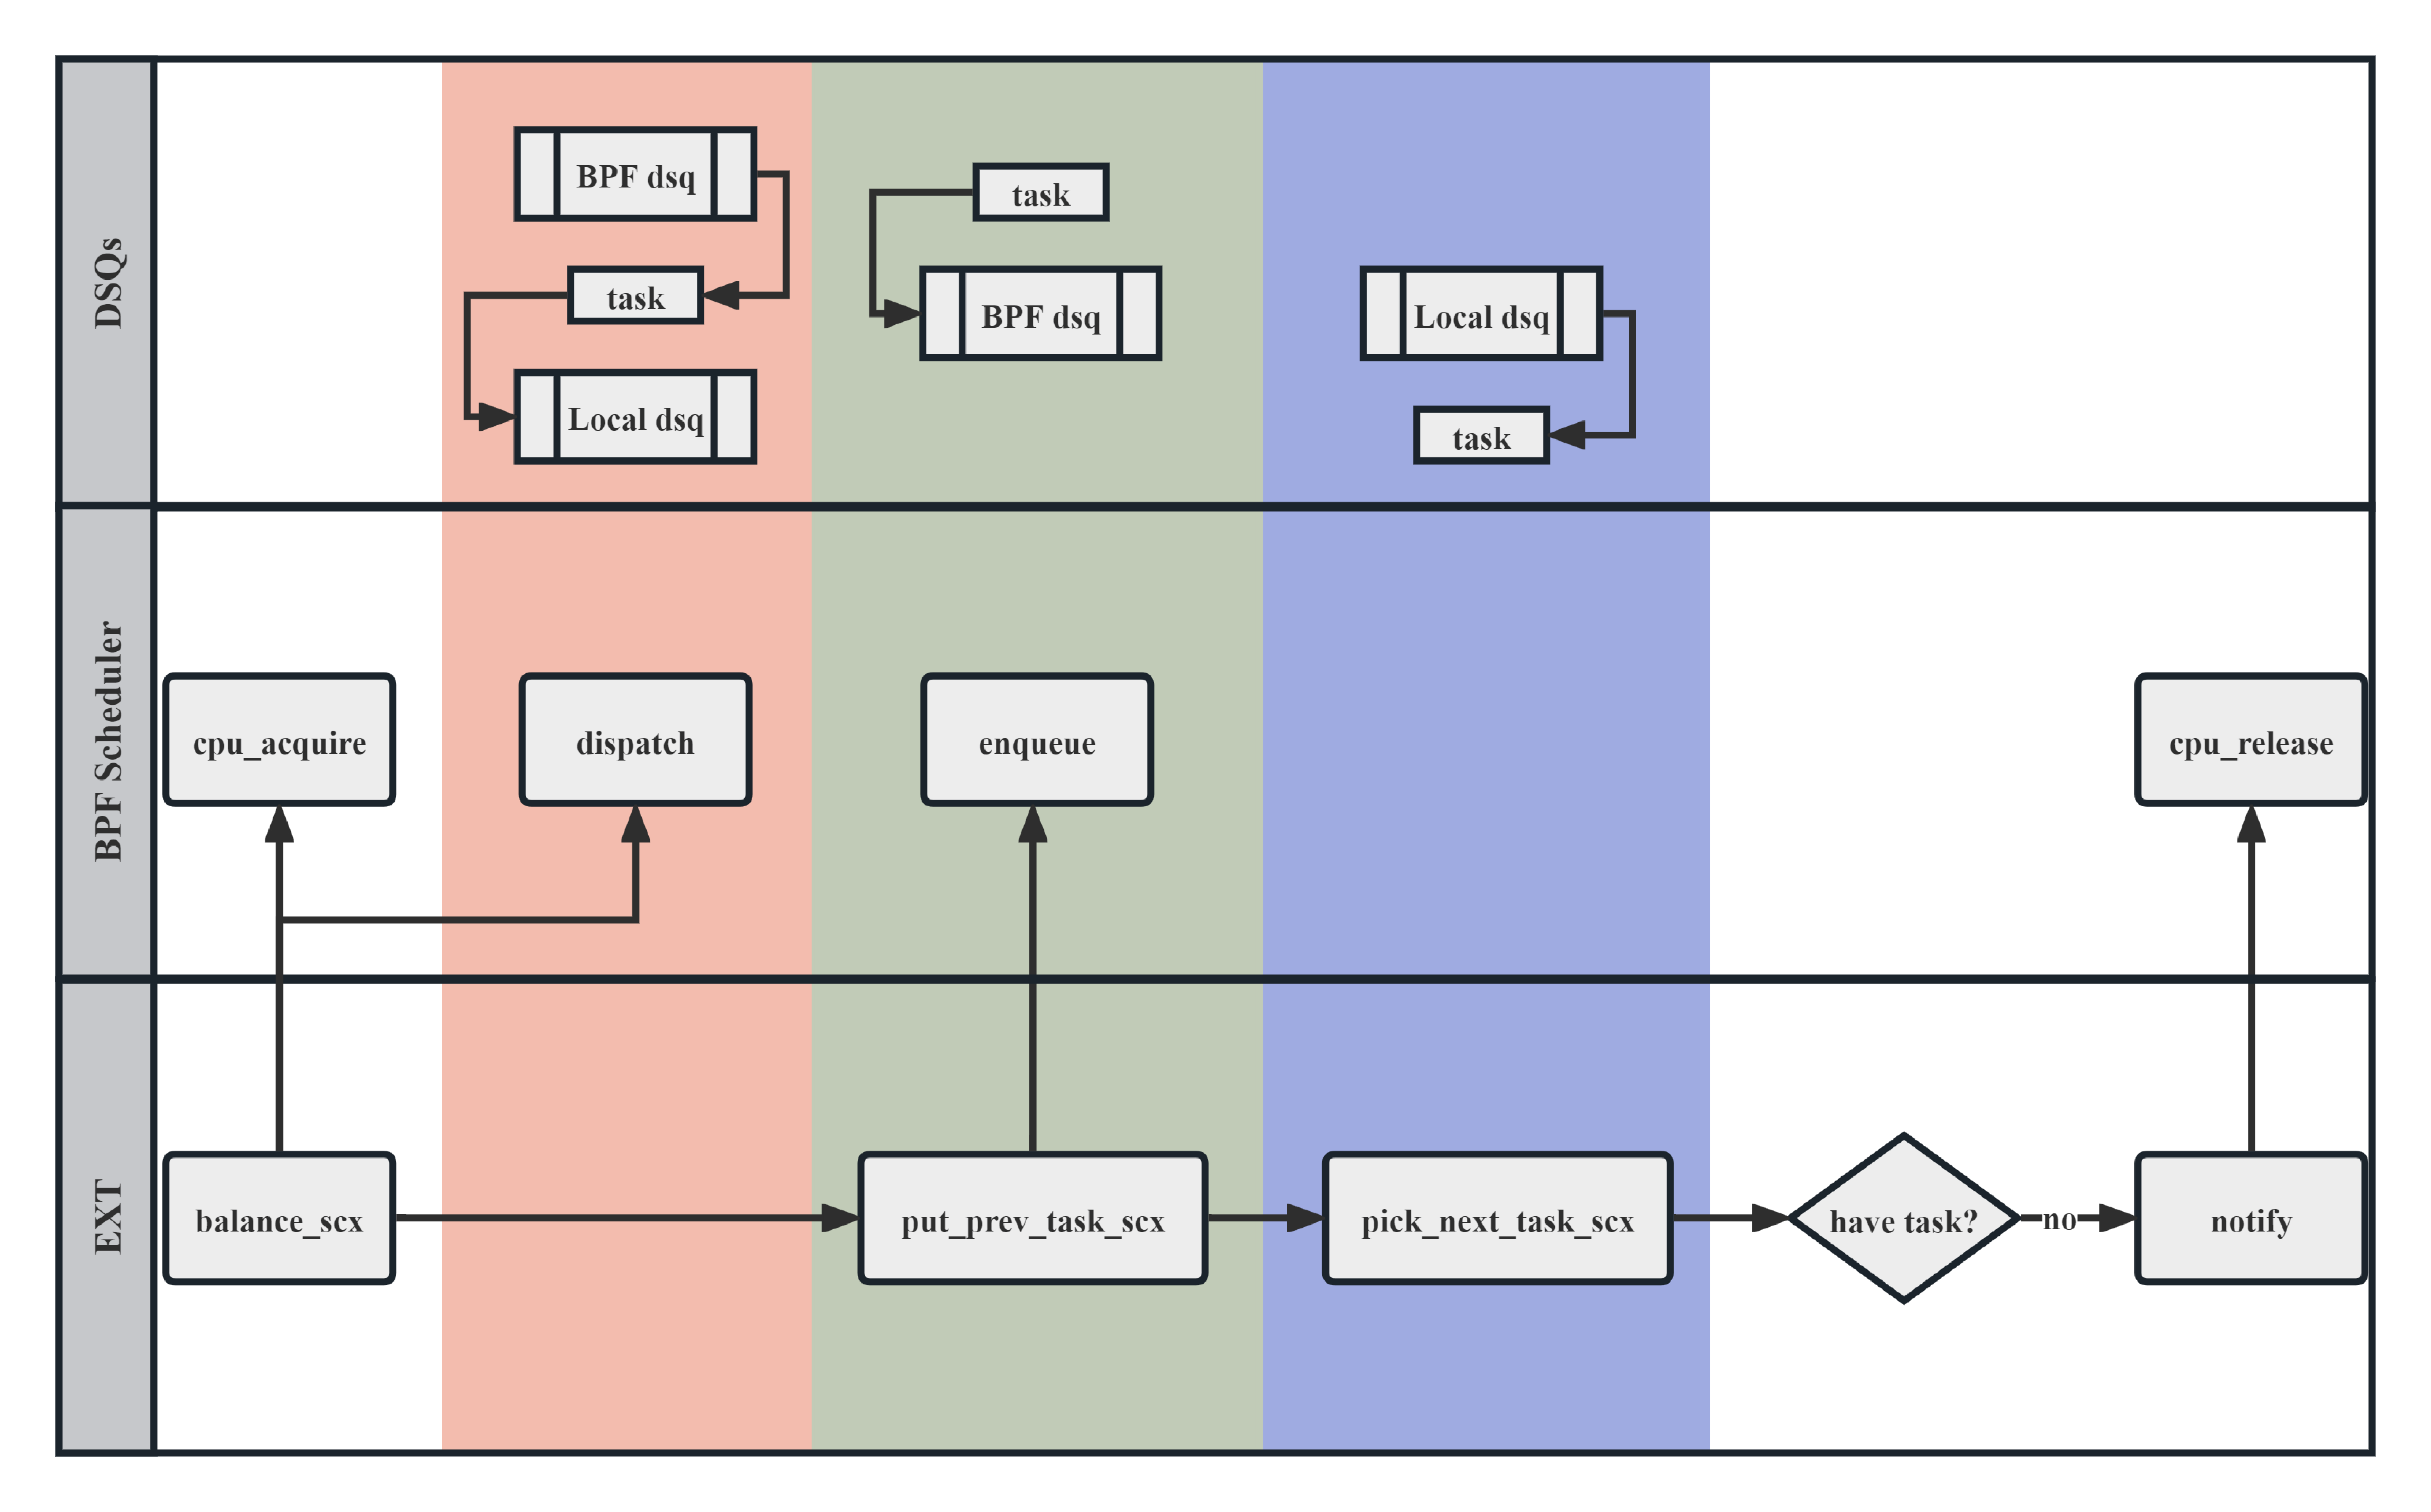
\includegraphics[width=0.85\textwidth]{ext_bpf}
    \bicaption{\quad Ext调度类与BPFScheduler协作}{\quad 
    Ext scheduling class cooperates with BPFScheduler}
    \label{fig:ext_bpf}
\end{figure}

\begin{itemize}
    \item \textbf{select\_cpu}:为唤醒的任务选择一个CPU。这一过程通常发送在SMP系统中,需要考虑任务的特性以及CPU的负载情况,选择的结果会影响到系统总体的性能,因此BPF所实现的逻辑不一定是最终的调度结果,实际的调度决策还会结合调度类本身的决策与BPF的决策。
    \item \textbf{enqueue}:处理任务的入队。调度类所管理的任务就绪时,会在入队的关键路径上触发BPF enqueue的执行,BPF中可将任务通过Helper函数发送到DSQ中,并进行后续的管理。
    \item \textbf{dequeue}:处理任务的出队。当需要对任务的调度属性,如优先级,进行修改时,便会触发任务出队逻辑,此时BPF中可以自定义优先级的更改逻辑,从而实现自定义的优先级功能。
    \item \textbf{tick}:处理任务滴答。Ext调度类在处理任务滴答时,触发此回调,并传入当前运行的任务。BPF Scheduler在tick中自定义任务滴答逻辑,如更新时间记账信息,同时,若在tick中将任务的时间片设置为0,则会在回调结束后直接触发一次dispatch,让CPU选择Ext调度队列中的另一个任务执行。
    \item \textbf{dispatch}:处理任务的调度。BPF可以通过创建DSQ来持有任务,同时每个CPU也拥有自己的Local DSQ来保存要执行的任务,当CPU的Local DSQ为空时,就会触发BPF的任务调度,期望从BPF的DSQ中获取将要执行的任务。BPF可以一次性调度多个任务,从而增加调度的效率,而任务的选择则完全由BPF程序决定。
    \item \textbf{runnable、running、stopping、quiescent}:追踪任务的状态。任务通常会在如下三种情况进入Runnable状态,首先是被唤醒时,如从等待IO的状态中恢复,其次是从其他CPU迁入时,以及从队列中暂移后恢复时,如修改任务优先级时,这些情况通过flag进行区分,并触发runnable的执行,quiescent的触发与上述时机完全相反,其他函数则在更细致的时机触发以反映任务的状态,其中running对应任务将要在CPU上运行时,stopping对应任务将要停止运行时。BPF通过这些函数来追踪任务的状态变化,从而辅助进行自定义的调度过程。
    \item \textbf{yield}:处理任务出让CPU资源。Linux提供了sched\_yield系统调用,允许任务主动放弃CPU资源,通常用于多线程中。sched\_yield并不保证线程组中的其他线程立即执行,而是将决策交给调度器,Sched Ext中此决策过程可完全由BPF程序实现。
    \item \textbf{cpu\_acquire、cpu\_release}:追踪调度类的CPU进出情况。当一个CPU对BPF Scheduler变为可用时,会触发cpu\_acquire,反之则触发cpu\_release。如当正在运行的EXT调度类的任务被更高优先级调度类的其他任务抢占时,当前CPU对于BPF Scheduler来说就变为不可用了。
    \item \textbf{init\_task、exit\_task}:追踪任务的创建与退出。调度类中每当有任务新创建或退出时触发,BPF可追踪这些事件,从而能够在BPF Scheduler中为每个任务定义额外的信息用于后续的调度过程。
\end{itemize}

BPF Schedueler为开发者提供了多样的模式来对Ext调度类进行定制。首先,最直接的方式是仅设置任务的调度类为Ext,由于并没有加载BPF Scheduler,Ext调度类会将任务委托给Fair调度类处理,这种模式主要用于对于任务调度状态的追踪。其次,开发者可以编写BPF Scheduler并加载到内核中,此时Ext调度类开始真正地调度任务,并可以根据开发者的需要来接管Fair调度类以及Idle调度类中的任务,从而方便地对系统中的主要任务进行管理。最后,开发者可以利用BPF程序的交互接口,进一步在用户态实现更复杂的调度逻辑,Sched Ext项目提供了一套基于Rust语言与Libbpf的用户态调度器开发框架,其实现的核心在于通过BPF Map和Ring Buffer在用户态代码与BPF Scheduler之间共享任务与调度事件,这种方式可以避免内核态以及BPF程序在表达能力上的限制,从而实现俄共灵活的调度策略。

\section{沙箱技术}

% 系统级沙箱(虚拟机),容器级沙箱(进程)
% 安全性: 虚拟机 > 沙箱
% - 容器类沙箱缺乏调度机制的支持,而对调度机制的修改需要更安全的沙箱环境来限制风险的传播

沙箱技术是一种安全机制,用于提供隔离的运行环境,以便在受限的环境中执行不受信任的程序。沙箱技术通常能够对程序所能使用的资源,如CPU、内存、网络等,并防止这些程序影响主机上其他程序。沙箱技术提供了安全运程序的基础,数据中心中常见的沙箱技术包括虚拟机技术与容器技术。

% TODO: 查看vm/370
虚拟机技术是数据中心应用广泛的沙箱技术,虚拟机指通过软硬件的手段,在已运行的系统中模拟出一个硬件环境,并能够支持运行其他系统。虚拟机技术最早提出于\citep{bugnion1997disco}, 用于解决操作系统迭代速度与硬件更新速度不匹配的问题,并希望依托虚拟设备与虚拟机环境,来提升操作系统的迭代速度。而随着虚拟化技术的不断发展,虚拟化开销也逐渐降低,其中软件上,从运行在裸金属上的Type 1虚拟化技术Xen\citep{barham2003xen},到能够将Linux转化为一个Hyeprvisor的Type 2虚拟化技术KVM\citep{kivity2007kvm},虚拟化软件技术的不断发展使得虚拟机的管理越来越简单,而在硬件上,基于SRIOV的设备直通手段\citep{dong2012high},让虚拟机能够直接接触物理设备,从而达到几乎与裸金属操作系统相近的性能。同时虚拟机具备较高的隔离性,能够较好的处理多租户场景下的安全性问题,以上这些为虚拟机在云厂商中较长时间的广泛使用提供了基础。

容器技术期望提供一种进程级别的沙箱,来隔离运行在同一系统上的不同进程。程序的执行依赖一定的运行环境,Linux早期的发展过程中,由于包管理工具的不成熟,使得不同程序之间会相互污染运行环境,造成程序的运行错误或失败,为解决此问题,Linux提供了chroot工具以及相关的系统调用,允许为程序设置不同的根目录,从而让不同的程序运行在满足各自运行环境的根目录中,解决相互之间的依赖污染问题。chroot实质是一种文件系统的隔离机制,而后在Linux的不断发展过程中,越来越多的隔离机制被实现,其中Cgroup与Namespace机制构成了现代容器技术的基础。Namespace技术提供了Mount、UTS、IPC、PID、Network及User等系统资源的隔离,使得容器中的进程认为自己运行在一个独立的系统环境中,而Cgroup技术则提供了CPU、Memory、BlkIO、NetIO、Devices等硬件资源的隔离,使得容器中的进程能够运行在一个受限制的硬件资源环境中。Overlayfs技术能够将多个目录文件叠加为一个统一的目录文件,并允许各层之间有不同的读写行为,同时借助COW(写时复制)来解决各层文件共享的问题,而这一技术为容器镜像技术提供了基础,而借助标准化的OCI镜像,容器得以方便地在不同的发行版、软件环境的Linux系统中传播。容器的易用性催生了容器编排技术,而以Kubernetes为主的容器编排技术在数据中心中占有越来越多的比例。

容器在本质上仍然是普通进程,因此在执行效率上高于虚拟机,但由于进程共享了相同的内核,因而不可避免地保有进程的安全问题,而这点在多租户场景的云环境中尤为凸显。现代容器技术提供了各种各样的手段提升容器的安全性,如限制容器中进程能够使用的系统调用等,然而这种方式牺牲了容器的通用性,容易导致部分容器的运行异常。安全容器的提出就试图解决这一问题,安全容器本质上是一个高度裁剪的虚拟机,运行着一个同样高度裁剪的内核,这样的处理大大精简了虚拟化环境,从而能够在提升虚拟机启动速度的同时,减少虚拟机本身的内存占用,同时,绝大多数的容器镜像都包含了一个较为完整的根文件系统,稍作处理后就可以作为一个虚拟机镜像来提供虚拟机使用。安全容器作为一种沙箱技术,结合了虚拟机的强隔离性与容器的易用性,在虚拟机监视器上,阿里的RunD\citep{li2022rund}、AWS的Firecraker\citep{agache2020firecracker}等轻量级虚拟机监视器大大降低了虚拟化的额外开销,而基于轻量级虚拟机技术所构建的安全容器如gVisor、KataContainer\citep{randazzo2019kata}等也逐渐在数据中心中应用。

\section{本章小结}

本章介绍了对任务调度机制进行定制的基础概念及本文使用的基于eBPF的定制Linux内核调度的方式。首先,介绍了Linux调度子系统的主要构成与工作方式,围绕Core调度框架、调度循环与任务抢占说明了调度子系统的核心过程。

随后,介绍了eBPF技术,说明其工作原理以及与其他内核功能扩展方式的差异,强调了eBPF在安全性、灵活性、可移植性以及性能上的特点。

然后,介绍了Sched Ext项目,分析了其主要组成的Ext调度类和BPF Scheduler的工作原理,Ext调度类的引入极大提高了Linux内核调度子系统在开发、测试、部署以及迭代的速度,使得在不同的混部场景下针对性地定制内核调度策略成为可能。

最后,介绍了沙箱技术,主要说明了常见的容器技术、虚拟机技术、安全容器技术三种沙箱技术,分析了不同沙箱技术的实现原理以及相互之间的优劣势。